\documentclass[12pt]{article}

\usepackage{amsmath}
\usepackage{amssymb}
\usepackage{amsthm}

\usepackage{xcolor}

%\usepackage[textheight=8.5in, margin=1.6in]{geometry}
\usepackage[total={6in,8in}]{geometry}

\usepackage{tikz}
%\usepackage{pgfplots}
\tikzstyle{ball} = [circle,shading=ball, ball color=black,
    minimum size=1mm,inner sep=1.3pt]
%\usetikzlibrary{arrows.meta}
%\tikzset{>={Latex[length=2mm,width=1.5mm]}}

%\usepackage{graphicx}

\usepackage{needspace}  % <-- to prevent bad pagebreak over environment titles
% Use:  \Needspace{3\baselineskip} before opening an environment

\usepackage{enumitem}
\setlist[enumerate]{leftmargin=*}

%\usepackage[colorlinks=true,citecolor=black,linkcolor=black,urlcolor=blue]{hyperref}

\newcommand{\N}{\mathbb{N}}
\newcommand{\Z}{\mathbb{Z}}
\newcommand{\Q}{\mathbb{Q}}
\newcommand{\R}{\mathbb{R}}
\newcommand{\C}{\mathbb{C}}
\newcommand{\T}{\mathbf{T}}
\newcommand{\tL}{\widetilde{L}}
\newcommand{\tF}{\widetilde{F}}
\newcommand{\tH}{\widetilde{H}}
\newcommand{\tb}{\tilde{\beta}}
\newcommand{\sn}{\mathfrak{S}}
\newcommand{\ve}{\varepsilon}
\newcommand{\proj}{\mathbb{P}}
\newcommand{\ips}[2]{\langle{#1}, {#2}\rangle}
\DeclareMathOperator{\tr}{tr}
\DeclareMathOperator{\Span}{\mathrm{Span}}
\DeclareMathOperator{\rk}{\mathrm{rank}}
\DeclareMathOperator{\trace}{\mathrm{tr}}
\DeclareMathOperator{\im}{\mathrm{im}}
\DeclareMathOperator{\Sym}{\mathrm{Sym}}
\DeclareMathOperator{\Hom}{\mathrm{Hom}}
\DeclareMathOperator{\diag}{\mathrm{diag}}
\DeclareMathOperator{\glb}{\mathrm{glb}}
\DeclareMathOperator{\lub}{\mathrm{lub}}
\DeclareMathOperator{\crit}{\mathcal{K}}
\DeclareMathOperator{\skel}{Skel}

\newtheorem{theorem}{Theorem}[section]
\newtheorem{lemma}[theorem]{Lemma}
\newtheorem{cor}[theorem]{Corollary}
\newtheorem{prop}[theorem]{Proposition}

\theoremstyle{definition}
\newtheorem{definition}[theorem]{Definition}
\newtheorem{example}[theorem]{Example}
\newtheorem{xca}[theorem]{Exercise}

\theoremstyle{remark}
\newtheorem{remark}[theorem]{Remark}

%\parskip = 0.05in
%\parindent = 0.0in

%\pagestyle{empty}

\begin{document}
\centerline{\sc notes on chip-firing for simplicial complexes}
\bigskip

Let~$\Delta$ be a~$d$-dimensional simplicial complex.  Denote its set
of~$i$-faces by~$F_i$, and define~$f_i:=|F_i|$.

\begin{definition}\label{def: spanning tree} 
  A {\em spanning tree of $\Delta$} is a $d$-dimensional subcomplex
  $\Upsilon\subseteq\Delta$ with $\skel_{d-1}(\Upsilon)=\skel_{d-1}(\Delta)$ and
  satisfying the three conditions:
  \begin{enumerate}[leftmargin=*]
    \item\label{sst1}  $\tH_d(\Upsilon)=0$;
    \item\label{sst2}  $\tb_{d-1}(\Upsilon)=0$;
    \item\label{sst3}  $f_d(\Upsilon) = f_d(\Delta)-\tb_d(\Delta)+\tb_{d-1}(\Delta)$.
  \end{enumerate}
  If $0\le k<d$, a \emph{$k$-dimensional (simplicial) spanning tree} of $\Delta$ is a spanning tree of
  the $k$-skeleton $\skel_{k}(\Delta)$.
  \end{definition}

\begin{prop}\label{prop: AC1}
Suppose that $\Delta$ is a $d$-dimensional simplicial complex. Then~$\Delta$ possesses a simplicial spanning tree if and only if $\tb_{d-1}(\Delta)=0$. We say that such complexes are \emph{acyclic in codimension 1}.
\index{simplicial complex!spanning trees of!and acyclicity}
\end{prop}
\begin{proof}
First suppose that $\Upsilon$ is a spanning tree of $\Delta$. Then $C_d(\Upsilon)\subset C_d(\Delta)$, $C_{d-1}(\Upsilon)=C_{d-1}(\Delta)$, and $\im(\partial_{\Upsilon,d})\subseteq\im(\partial_{\Delta,d})$. It follows that there is a surjection
\[
\tH_{d-1}(\Upsilon)=C_{d-1}(\Upsilon)/\im(\partial_{\Upsilon,d})\twoheadrightarrow 
C_{d-1}(\Delta)/\im(\partial_{\Delta,d})=\tH_{d-1}(\Delta).
\]
Since $\tH_{d-1}(\Upsilon)$ is finite, it follows that $\tH_{d-1}(\Delta)$ is also finite, hence $\tb_{d-1}(\Delta)=~0$.

Now suppose that $\Delta$ is acyclic in codimension 1. To construct a spanning tree, start with $\Upsilon=\Delta$. If $\tH_d(\Upsilon)=0$, then $\Upsilon$ is a spanning tree, and we are done. If not, then there is an integer-linear combination of facets $\sigma_i$ in the kernel of $\partial_d$:
\[
a_1\sigma_1+a_2\sigma_2+\cdots+a_k\sigma_k,
\]
where we assume that $a_1\ne 0$. If we work over the rational numbers, then we may assume $a_1=1$. Still working over the rationals, we see that 
\[
\partial_d(\sigma_1)=-\sum_{i=2}^ka_i\partial_d(\sigma_i).
\]
Hence, if we remove the facet $\sigma_1$ from $\Upsilon$, we obtain a smaller subcomplex $\Upsilon'$ without changing the image of the rational boundary map: $\im(\partial_{\Upsilon,d})=\im(\partial_{\Upsilon',d})$. It follows from rank-nullity that
\[
\tb_d(\Upsilon')=f_d(\Upsilon')-\rk\,\im(\partial_{\Upsilon',d})=f_d(\Upsilon)-1-\rk\,\im(\partial_{\Upsilon,d})
=\tb_d(\Upsilon)-1,
\]
and $\tb_{d-1}(\Upsilon')=\tb_{d-1}(\Upsilon)=0$. Continuing to remove facets in this way, we eventually obtain a spanning tree of $\Delta$.
\end{proof}

\begin{cor}\label{cor: AC1} If~$0\leq i\leq d$, then~$\Delta$ has
  an~$i$-dimensional spanning tree if and only if~$\tb_{i-1}(\Delta)=0$.
\end{cor}
\begin{proof} This follows from the previous proposition
  since~$\tb_{i-1}(\skel(\Delta))=\tb_{i-1}(\Delta)$.
\end{proof}

\begin{prop}\label{prop: unique tree} If~$\Delta$ has a unique~$d$-dimensional spanning tree~$\Psi$,
  then~$\Delta=\Psi$.
\end{prop}
\begin{proof}
  To come.
\end{proof}

Let~$0\leq i\leq d$.  The {\em $i$-th tree number} for~$\Delta$ is
\[
  \tau_i:=\tau_i(\Delta):=\sum_{\Psi}|H_{i-1}(\Psi)|^2,
\]
where the sum is over all~$i$-dimensional spanning trees of~$\Delta$.

\begin{cor}\label{cor: tree number}
  $\tau_d(\Delta)=1$ if and only if~$\Delta$ is a tree
  and~$\tH_{d-1}(\Delta)=0$, i.e., if and only
  if~$\tH_d(\Delta)=\tH_{d-1}(\Delta)=0$.
\end{cor}
\begin{proof}
  This follows directly from the definition of~$\tau_d(\Delta)$ and
  Proposition~\ref{prop: unique tree}.
\end{proof}

Suppose that $\tb_{i-1}(\Delta)=0$.  It follows that~$\Delta$ has an
$i$-dimensional spanning tree~$\Upsilon$. Let
\[
  \tF_i:=F_i(\Delta)\setminus F_i(\Upsilon),
\]
the $i$-faces of $\Delta$ not contained in $\Upsilon$, and let $\tL_i$ be the
$i$-Laplacian of~$\Delta$ with the rows and columns corresponding to faces in
$F_i(\Upsilon)$ removed.

\begin{theorem}[Duval, Klivans, Martin]\label{thm: simplicial matrix-tree}
  \leavevmode
\begin{enumerate}[label={\rm (\roman*)}]
  \item\label{thm: smt1}  If $\tH_{i-1}(\Upsilon)=0$, there is an isomorphism
    \[
      \psi\colon\crit_i(\Delta)\to \Z\tF_i/\im(\tL_i),
    \]
    defined by dropping $i$-faces
    of $\Upsilon$:   if
    $c=\sum_{f\in F_i(\Delta)}c_f\cdot f\in\ker\partial_i$ represents an element
    of $\crit_i(\Delta)$, then 
    \[
      \psi(c)=\sum_{f\in\tF_i}c_f\cdot f\ \bmod\im(\tL_i).
  \]
\item\label{thm: smt2} (Simplicial matrix-tree theorem)
  \[
    \tau_{i+1}=\frac{|\tH_{i-1}(\Delta)|^2}{|\tH_{i-1}(\Upsilon)|^2}\,\det(\tL_i).
  \]
\end{enumerate}
\end{theorem}

\begin{definition} Let~$0\leq i\leq d$.  The {\em $i$-th positive kernel}
  for~$\Delta$ is the pointed cone
  \[
    \ker^{+}L_i:=\left\{ D\in \Z F_i: D(f)\geq0\ \text{for all $f\in F_i$}
    \right\}.
  \]
  Fixing an ordered Hilbert basis~$H_i=(h_1,\dots,h_{\ell})$ for
  $\ker^{+}L_i\cap\Z^{f_i(\Delta)}$, define the {\em degree}
  of~$D\in\Z F_i$ by
  \[
    \deg(D):= (D\cdot h_1,\dots, D\cdot h_{\ell})
  \]
  where~$D\cdot h_j:=\sum_{f\in F_i}D(f)h_j(f)$.  
  We say~$d\in\Z^{\ell}$ is a {\em winning degree (in dimension~$i$)} if each~$D\in \Z F_i$
  with~$\deg(D)\geq d$ is winnable.
\end{definition}

\begin{prop}\label{prop: deg 0 iso} For $0\leq i\leq d$, 
\[
  (\ker L_i)^{\perp}/\im(L_i)\approx \T(\crit_i(\Delta)).
\]
This says the group of~$i$-chains of degree~$0$ modulo firing rules is
isomorphic to the torsion part of the~$i$-th critical group
of~$\Delta$.\footnote{Need to say why the perp is the group of~$i$-chains of
degree~$0$.}
\end{prop}

\begin{theorem} Suppose that~$\tau_d(\Delta)=1$.  Then~$0$ is a winning degree in
  dimension~$d-1$ if and only if~$\tH^d(\Delta)$ is free. (NOTE: check on
  whether reduced cohomology is important here.)
\end{theorem}
\begin{proof} Since~$\tau_d(\Delta)=1$, by Proposition~\ref{cor: tree number},
  we have~$\tH_d(\Delta)=\tH_{d-1}(\Delta)=0$.  Thus,~$\partial_d$ is injective,
  and~$\im\partial_d=\ker\partial_{d-1}$.

  First suppose that~$\tH^d(\Delta)$ is free.  To show~$0$ is a winning degree
  in dimension~$d-1$, we must show~$\crit_{d-1}(\Delta)$ is also torsion-free.
  So let~$\alpha\in\ker\partial_{d-1}$ and suppose there exists an
  integer~$n>0$ such that~$n\alpha\in\im(L_{d-1})$.  So there exists~$\beta\in
  C_{d-1}(\Delta)$ such that
  \[
    n\alpha=L_{d-1}\beta=\partial_d\partial_d^t\beta.
  \]
  Since~$\tH_{d-1}(\Delta)=0$,
  there exists~$\gamma\in C_d(\Delta)$ such that~$\partial_d\gamma=\alpha$.  
  Since~$\partial_d$ is injective,~$n\gamma=\partial_d^t\beta$.
  Since~$\tH^d(\Delta)=C^d(\Delta)/\im\partial_d^t=0$, it follows
  that~$\gamma=\im\partial_d^t$, and hence,~$\alpha\in\im L_{d-1}$, as required.

  Conversely, suppose that~$0$ is a winning degree in dimension~$d-1$.  We would
  like to show that~$\tH^d(\Delta)$ is free.  So
  say~$n\sigma=\partial_d^t\mu\in\im\partial_d^t$ for some~$\sigma\in
  C^d(\Delta)$ and some integer~$n>0$
  It follows that~$n\partial_d\sigma=0$ as an element of~$\crit_{_d-1}(\Delta)$.
  However,~$\crit_{d-1}(\Delta)$ is torsion-free.
  So~$\partial_d\sigma=L_{d-1}\nu=\partial_d\partial_d^t\nu$ for some~$\nu\in
  C_{d-1}(\Delta)$.  Since~$\partial_d$ is injective, it follows
  that~$\sigma=\partial_d^t\nu$.
\end{proof}

\begin{example}
  Figure~\ref{fig: real projective plane} illustrates a~$2$-dimensional
  complex~$P$ which is a triangulation of the real projective plane.  We
  have~$\tH_0(P)=\tH_2(P)=0$, and~$\tH_1(P)\approx\Z/2\Z$.  From the definition
  of the tree number,~$\tau_2(P)=4$, and it follows from the matrix-tree theorem
  that~$\det(\tL_0)=4$ with respect to any~$1$-dimensional spanning tree
  of~$P$.  (There are~$6^4$ such spanning trees since the~$1$-skeleton
  of~$P$ is the completer graph~$K_6$.)  The
  cycle~$C:=\overline{01}+\overline{12}-\overline{02}$ has degree~$(0,0,0,0,0)$ but
  is not winnable.  We have~$\crit_1(P)\approx\Z/2\Z\times\Z/2\Z$, and
  hence~$2C$ is winnable.
\begin{figure}[ht] 
  \centering
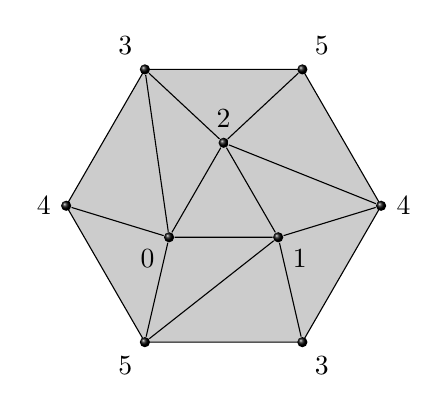
\begin{tikzpicture}
  \def\r{2.0cm}
  \draw[fill=gray!40] ({\r*cos(0*60)},{\r*sin(0*60)})--({\r*cos(1*60)},{\r*sin(1*60)})--({\r*cos(2*60)},{\r*sin(2*60)})--({\r*cos(3*60)},{\r*sin(3*60)})--({\r*cos(4*60)},{\r*sin(4*60)})--({\r*cos(5*60)},{\r*sin(5*60)})--({\r*cos(6*60)},{\r*sin(6*60)});
  
  \draw ({\r*cos(0*60},{\r*sin(0*60)}) node[label=0*60:{$4$},ball] (1) {};
  \draw ({\r*cos(1*60},{\r*sin(1*60)}) node[label=1*60:{$5$},ball] (2) {};
  \draw ({\r*cos(2*60},{\r*sin(2*60)}) node[label=2*60:{$3$},ball] (3) {};
  \draw ({\r*cos(3*60},{\r*sin(3*60)}) node[label=3*60:{$4$},ball] (11) {};
  \draw ({\r*cos(4*60},{\r*sin(4*60)}) node[label=4*60:{$5$},ball] (22) {};
  \draw ({\r*cos(5*60},{\r*sin(5*60)}) node[label=5*60:{$3$},ball] (33) {};

  \def\s{0.8cm}
  \draw ({\s*cos(210},{\s*sin(210)}) node[label=210:{$0$},ball] (4) {};
  \draw ({\s*cos(-30},{\s*sin(-30)}) node[label=-30:{$1$},ball] (5) {};
  \draw ({\s*cos(90},{\s*sin(90)}) node[label=90:{$2$},ball] (6) {};

  \draw (22)--(4);
  \draw (22)--(5)--(33);
  \draw (5)--(1)--(6)--(2);
  \draw (6)--(3)--(4)--(11);
  \draw (6)--(4)--(5)--(6);
\end{tikzpicture}
\caption{A triangulation of the real projective plane, $\R\proj^2$.}\label{fig:
real projective plane} 
\end{figure}
\end{example}

\noindent{\bf Question.}  Can we find an example where~$\tau_d(\Delta)=1$
and~$0$ is not a winning degree in dimension~$d-1$?  The~$2$-dimensional
chessboard complex is an example of a non-tree for which~$0$ is a winning degree
in dimension~$1$.
\end{document}

# The following proof has fatal flaws.
\begin{prop}
  Suppose $\tH_{d-2}(\Delta)=0$ and~$0$ is a winning degree in dimension~$d-1$.
  Then~$\tau_d(\Delta)=1$, and hence~$\Delta$ is a tree.
\end{prop}
\begin{proof}
  Since~$\tH_{d-2}(\Delta)=0$, it follows that~$\tb_{d-2}(\Delta)=0$, and
  hence~$\Delta$ has a~$(d-2)$-dimensional spanning tree~$\Upsilon$.  Further,
  since~$\Upsilon$ and~$\Delta$ have the same~$(k-1)$-skeleton, 
  we have~$0=H_{d-2}(\Delta)=H_{d-1}(\Upsilon)$.  
  Since~$0$ is a winning degree in dimension~$d-1$, Proposition~\ref{prop: deg 0
  iso} implies that $\crit_{d-1}(\Delta)$ is a free module.
  It then
  follows from Theorem~\ref{thm: simplicial matrix-tree}, part~\ref{thm: smt1}
  that~$\det(\tL_{d-1})=1$, and thus, using the fact that~$\tH_{d-2}(\Delta)=0$,
  the simplicial matrix-tree theorem implies 
  \[
  \tau_{d}=\frac{|\tH_{d-2}(\Delta)|^2}{|\tH_{d-2}(\Upsilon)|^2}\,\det(\tL_{d-1})=1.
  \]
\end{proof}
